\chapter{Malkovri la bazajn primitivojn}
\label{bazo}

{ }\hfill\textbf{Nivelo:} komencanto\\ \\
\noindent
Por movi la testudon sur la ekrano, oni uzas anta^udifinitajn
komandojn nomatajn \og primitivoj\fg.  En tiu ^ci ^capitro, ni
malkovros kelkajn bazajn primitivojn ebligantajn gvidi la testudon.
\section{Novaj primitivoj uzotaj:}
\noindent \begin{enumerate}
\item  \texttt{an nombro}\hspace {4cm } \textcolor{red}{ \texttt{an 50}}\\
  Anta^uenigi la testudon je la nombro de testudaj pa^soj indikitaj.
\item  \texttt{man nombro}\hspace {4cm } \textcolor{red}{ \texttt{man 100}}\\
  Malanta^uenigi la testudon je la nombro de testudaj pa^soj indikitaj.
\item  \texttt{dn nombre}\hspace {4cm } \textcolor{red}{\texttt{dn 90}}\\
  La testudon turni dekstren je l' angulo indikita.
\item  \texttt{mdn nombre}\hspace {4cm } \textcolor{red}{ \texttt{mdn 45}}\\
  La testudon turni maldekstren je l' angulo indikita.
\item  \texttt{ev}\hspace {4cm } \textcolor{red}{ \texttt{ev}}\\
  Vi^si l' ekranon kaj remeti la testudon centren de l' ekrano.
\item  \texttt{tdm}\hspace {4cm } \textcolor{red}{ \texttt{tdm}}\\
  La testudo esti videbla sur l' ekrano.
\item  \texttt{tdk}\hspace {4cm } \textcolor{red}{ \texttt{tdk}}\\
  Testudon ka^si.  Eble ebligas grafiki pli rapide.
\item  \texttt{l}\hspace {4cm } \textcolor{red}{ \texttt{l}}\\
  Levi la krajonon.  La testudo ne lasas ^spuron post si kiam ^gi movi^gas.
\item  \texttt{ml}\hspace {4cm } \textcolor{red}{ \texttt{ml}}\\
  Mallevi la krajonon.  La testudo skribas kiam ^gi movi^gas.
\item  \texttt{ripetu nombro listo}\hspace {4cm } \textcolor{red}{ \texttt{ripetu 5 [an 50 dn 45]}}\\
  Ripeti l' instrukciojn enhavatajn en la listo je la nombro de fojoj indikita.
\end{enumerate}
\section{Desegni regulan plurlateron}
\noindent ^Ci tie, ni lernos desegni kvadraton, egallateran
trilateron, regulan kvinlateron, ktp.
\subsection{La kvadrato}
\begin{center}
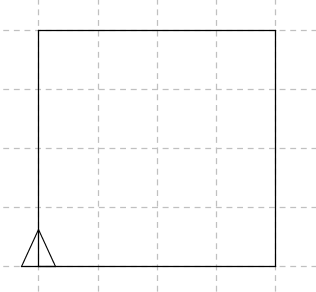
\includegraphics{bildoj/bases-carre.png}
\end{center}
\noindent Unu reta ^celo reprezentas 50 testudajn pa^sojn.  Por
desegni la apudan kvadraton, oni do tajpu:
\begin{verbatim}
an 200 dn 90 an 200 dn 90 an 200 dn 90 an 200 dn 90
\end{verbatim}
Oni rimarku ke oni ripetas $4$ fojojn la saman instrukcion, do jen
sintakso pli rapida:
\begin{verbatim}
ripetu 4 [an 200 dn 90]
\end{verbatim}
\subsection{La egallatera trilatero}
\begin{center}
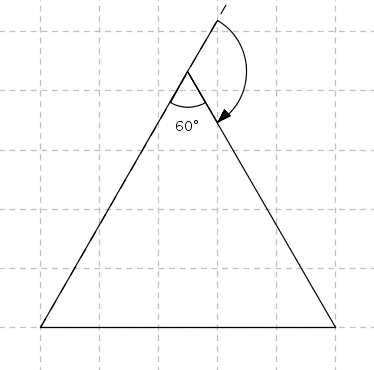
\includegraphics{bildoj/bases-triangle.png}
\end{center}
\noindent ^Ci tie, ^celo reprezentas 30 testudpa^sojn.  Ni vidos kiel
desegni tiun egallateran trilateron kun lateroj de 150 testudpa^soj.
La instrukcio similos ion tian:
\begin{verbatim}
ripetu 3 [an 150 dn ...]
\end{verbatim}
Restas kalkuli la bonan angulon.  En egallatera trilatero, l' anguloj
havas ^ciuj 60 gradojn.  ^Car la testudo turni^gas ekster la
trilatero, l' angulo validas $180-60=120$ gradojn.  L' instrukcio estas
do:
\begin{verbatim}
ripetu 3 [an 150 dn 120]
\end{verbatim}
\subsection{La seslatero}
\begin{center}
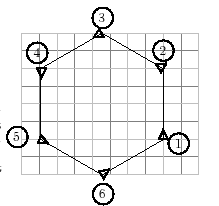
\includegraphics{bildoj/bases-hexagone.png}
\end{center}
\noindent ^Ci tie, ^celo reprezentas 20 testudpa^sojn.

\begin{verbatim}
ripetu 6 [an 80 dn ...]
\end{verbatim}

Oni rimarku ke dum ^gia movi^go, la testudo efektivigas kompletan
turni^gon (^gi ekiras adresita al supro, fine ^gi revenas en tiun
saman pozicion).  Tiu turni^go je 360 gradoj efektivi^gos post 6
eta^goj.  Tial, je ^ciu fojo, ^gi turni^gas je
${360} / {6}=60$\degre.

L' instrukcio estu do: \texttt{ripetu 6 [an 80 dn 60]}

\subsection{Desegni regulan plurlateron ^generale}
\noindent Efektive, ripetante la malgrandan pensadon anta^uan, oni
rimarku ke, por desegni plurlateron je $n$ lateroj, l' angulon oni
kalkulu per divido de $360$ per $n$.  Por ekzemplo:
\begin{itemize}
\item Por grafiki regulan kvinlateron je latero $100$:
\begin{verbatim}
ripetu 5 [an 100 dn 72]    (360:5=72)
\end{verbatim}
\item Por grafiki regulan na^ulateron je latero $20$:
\begin{verbatim}
ripetu 9 [an 20 dn 40]    (360:9=40)
\end{verbatim}
\item Por grafiki regulan ee... 360-lateron je latero $2$ (^gi ja
  similas cirklon!):
\begin{verbatim}
ripetu 360 [an 2 dn 1]  
\end{verbatim}
\item Por grafiki seplateron je latero $120$:
\begin{verbatim}
ripetu 7 [an 120 dn 360/7]
\end{verbatim}
\end{itemize}

\section{Registri proceduron}
\noindent Por ne devi retajpi ^ciufoje l' instrukciojn por desegni
kvadraton, trilateron... oni povas difini personajn komandojn nomatajn
\og proceduroj\fg.  Proceduro komenci^gas per la ^cefvorto
\texttt{por} kaj fini^gas per la ^cefvorto \texttt{fino}.  Oni
malfermu la redaktilon kaj tajpu ekzemple

\begin{verbatim}
por kvadrato
ripetu 4 [an 100 dn 90]
fino
\end{verbatim}

Poste oni fermu l' redaktilon registrante l' modifojn per klaki la
butonon testudo.  Nun je ^ciu fojo kiam oni tajpas \texttt{kvadrato},
kvadrato aperas sur l' ekrano!

\section{Ekzerco...}
\noindent
Malgranda reta ^celo reprezentas $10$ testudpa^sojn.

Provu realigi la grafikon malsupran per difini ok procedurojn:
\begin{itemize}
\item Proceduron \og \texttt{kvadrato}\fg{} kiu grafikos la bazan
  kvadraton de la domo.
\item Proceduron \og \texttt{tri}\fg{} kiu grafikos l' egallateran
  trilateron kiu reprezentos la tegmenton doman.
\item Proceduron \og \texttt{pordo}\fg{} kiu grafikos l' ortangulon
  reprezentantan la pordon.
\item Proceduron \og \texttt{kam}\fg{} kiu grafikos la kamentubon.
\item Proceduron \og \texttt{mov1}\fg{} kiu ebligos la testudon
  movi^gi de pozicio A al pozicio B.
\item Proceduron \og \texttt{mov2}\fg{} kiu ebligos la testudon
  movi^gi de pozicio B al pozicio C.
\item Proceduron \og \texttt{mov3}\fg{} kiu ebligos la testudon
  movi^gi de pozicio C al pozicio D.  (Atentu: eble necesos levi la
  testudan krajonon...)
\item Proceduron \og \texttt{domo}\fg{} kiu ebligos grafiki la domon
  tutan helpe de ^ciuj aliaj proceduroj.
\end{itemize}
\label{maison}
\begin{center}
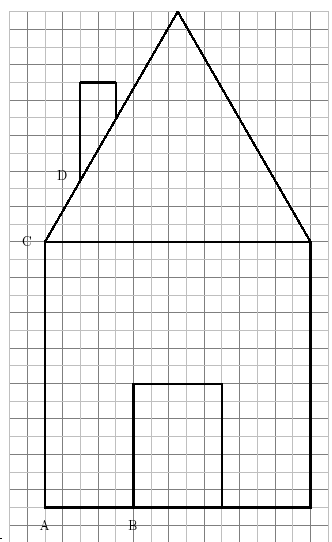
\includegraphics[scale=0.6]{bildoj/bases-maison.png}
\end{center}
